%
% main.tex
%
% Copyright (C) 2023 by Gabriel Mariano Marcelino.
%
% Towards the Conception of GNSS Networks Based on Small Satellites
%
% This work is licensed under the Creative Commons Attribution-ShareAlike 4.0
% International License. To view a copy of this license,
% visit http://creativecommons.org/licenses/by-sa/4.0/.
%

%
% \brief Main file.
%
% \author Gabriel Mariano Marcelino <gabriel.mm8@gmail.com>
%
% \version 1.0.0
%
% \date 2023/09/07
%

\documentclass{beamer}

\usepackage{presentation}

\title[Presentation]{Towards the Conception of GNSS Networks Based on Small Satellites}
\author[Gabriel M. Marcelino]{Gabriel Mariano Marcelino}
\institute[]{SpaceLab - UFSC}
\date{2023 September 11}

\hypersetup
{
    pdfauthor   = {Gabriel Mariano Marcelino},
    pdfsubject  = {PhD Thesis Qualification},
    pdftitle    = {Towards the Conception of GNSS Networks Based on Small Satellites},
    pdfkeywords = {Embedded Systems,GNSS,Satellites}
}

\begin{document}

    %
% titlepage.tex
%
% Copyright (C) 2023 by Gabriel Mariano Marcelino.
%
% Towards the Conception of GNSS Networks Based on Small Satellites
%
% This work is licensed under the Creative Commons Attribution-ShareAlike 4.0
% International License. To view a copy of this license,
% visit http://creativecommons.org/licenses/by-sa/4.0/.
%

%
% \brief Title page.
%
% \author Gabriel Mariano Marcelino <gabriel.mm8@gmail.com>
%
% \version 1.0.0
%
% \date 2023/09/07
%

\begin{frame}
    \titlepage
\end{frame}

    %
% contents.tex
%
% Copyright (C) 2023 by Gabriel Mariano Marcelino.
%
% Towards the Conception of GNSS Networks Based on Small Satellites
%
% This work is licensed under the Creative Commons Attribution-ShareAlike 4.0
% International License. To view a copy of this license,
% visit http://creativecommons.org/licenses/by-sa/4.0/.
%

%
% \brief Table of contents.
%
% \author Gabriel Mariano Marcelino <gabriel.mm8@gmail.com>
%
% \version 1.0.0
%
% \date 2023/09/07
%

\begin{frame}
    \frametitle{Summary}
    \tableofcontents
\end{frame}


    \section{Introduction}

        %
% introduction.tex
%
% Copyright (C) 2023 by Gabriel Mariano Marcelino.
%
% Towards the Conception of GNSS Networks Based on Small Satellites
%
% This work is licensed under the Creative Commons Attribution-ShareAlike 4.0
% International License. To view a copy of this license,
% visit http://creativecommons.org/licenses/by-sa/4.0/.
%

%
% \brief Introduction slides.
%
% \author Gabriel Mariano Marcelino <gabriel.mm8@gmail.com>
%
% \version 1.0.0
%
% \date 2023/09/07
%

\begin{frame}{Introduction}

    \begin{columns}[t]
        \begin{column}[t]{0.6\textwidth}
            \begin{itemize}
                \item Camera payload for small satellites (CubeSats)
                \vspace{0.5cm}
                \item Project name: ``\textit{SLCam}'' (SpaceLab Camera)
                \vspace{0.5cm}
                \item Main objective: Take pictures of the Earth from space
            \end{itemize}
        \end{column}
        \begin{column}[t]{0.4\textwidth}
        \end{column}
    \end{columns}

\end{frame}


    \section{Related Projects and References}

        %
% related-work.tex
%
% Copyright (C) 2023 by Gabriel Mariano Marcelino.
%
% Towards the Conception of GNSS Networks Based on Small Satellites
%
% This work is licensed under the Creative Commons Attribution-ShareAlike 4.0
% International License. To view a copy of this license,
% visit http://creativecommons.org/licenses/by-sa/4.0/.
%

%
% \brief Related work slides.
%
% \author Gabriel Mariano Marcelino <gabriel.mm8@gmail.com>
%
% \version 1.0.0
%
% \date 2023/09/07
%


\begin{frame}{Related Work}


\end{frame}


    \section{Problem Discussion}

        %
% problem.tex
%
% Copyright (C) 2023 by Gabriel Mariano Marcelino.
%
% Towards the Conception of GNSS Networks Based on Small Satellites
%
% This work is licensed under the Creative Commons Attribution-ShareAlike 4.0
% International License. To view a copy of this license,
% visit http://creativecommons.org/licenses/by-sa/4.0/.
%

%
% \brief Problem discussion slides.
%
% \author Gabriel Mariano Marcelino <gabriel.mm8@gmail.com>
%
% \version 1.0.0
%
% \date 2023/09/09
%

\begin{frame}{Problem Discussion}


\end{frame}

\begin{frame}{Timing Precision}


\end{frame}

\begin{frame}{Ionospheric Delay}

    \begin{columns}[t]
        \begin{column}[t]{0.5\textwidth}
            \begin{itemize}
                \item .
            \end{itemize}
        \end{column}
        \begin{column}[t]{0.5\textwidth}
            \begin{figure}[!ht]
                \begin{center}
                    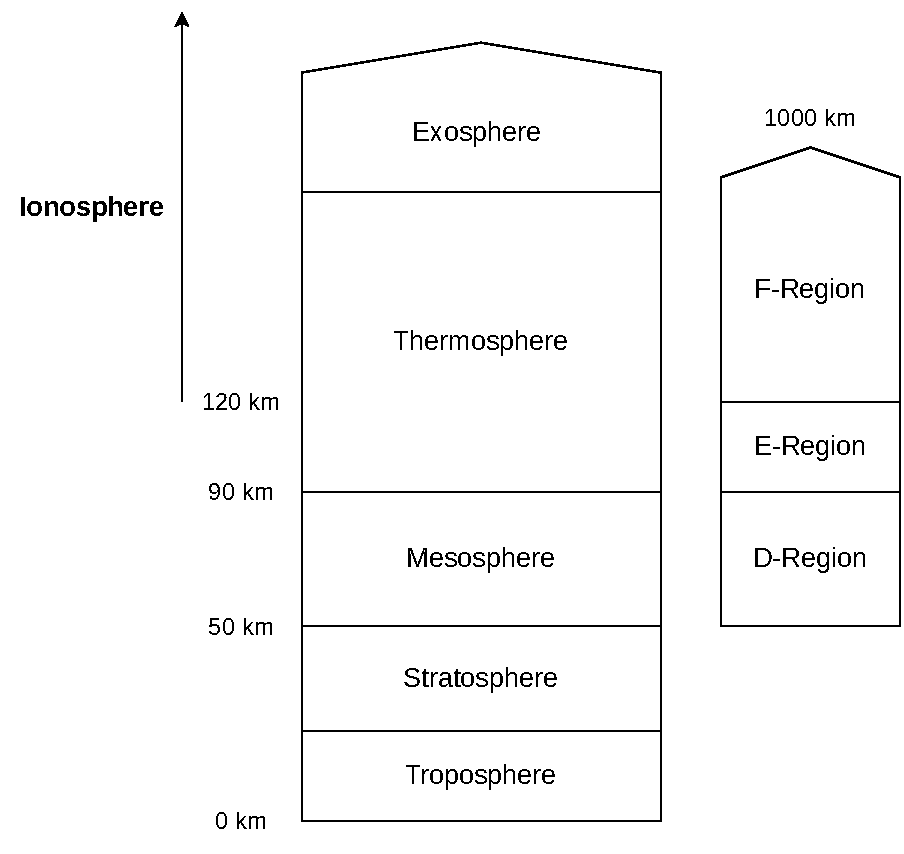
\includegraphics[width=\columnwidth]{figures/atmosphere-model}
                \end{center}
            \end{figure}
        \end{column}
    \end{columns}

\end{frame}

\begin{frame}{Telecommunication Analysis}


\end{frame}

\begin{frame}{Power Budget Analysis}


\end{frame}

\begin{frame}{Orbit Analysis}


\end{frame}


    \section{Proposed Work}

        %
% proposed.tex
%
% Copyright (C) 2023 by Gabriel Mariano Marcelino.
%
% Towards the Conception of GNSS Networks Based on Small Satellites
%
% This work is licensed under the Creative Commons Attribution-ShareAlike 4.0
% International License. To view a copy of this license,
% visit http://creativecommons.org/licenses/by-sa/4.0/.
%

%
% \brief Proposed work slides.
%
% \author Gabriel Mariano Marcelino <gabriel.mm8@gmail.com>
%
% \version 1.0.0
%
% \date 2023/09/09
%

\begin{frame}{Proposed Work}

    \begin{itemize}
        \item .
        \item Orbit study
        \item Communication study
        \item Required power budget
        \item Possible technical solutions
        \item Proposed experiment
    \end{itemize}

\end{frame}

\begin{frame}{Orbit Study}

    \begin{itemize}
        \item Current GNSS networks operate mostly in MEO
        \vspace{0.1cm}
        \item Higher altitudes require more robust components
        \vspace{0.1cm}
        \item Lower altitudes make the design of onboard electronics easier
        \vspace{0.1cm}
        \item To achieve the same coverage as a constellation operating at a higher altitude, lower altitudes require a larger number of satellites in the constellation
        \vspace{0.1cm}
        \item In addition to complexity and the number of satellites, the cost and ease of launching and replacement of the fleet should also be taken into account
        \vspace{0.1cm}
        \item \textbf{Trade-off}: Higher altitudes with fewer but more complex satellites $\times$ Lower altitudes with more but simpler satellites
    \end{itemize}

\end{frame}

\begin{frame}{Orbit Analysis}

    \begin{figure}[!ht]
        \begin{center}
            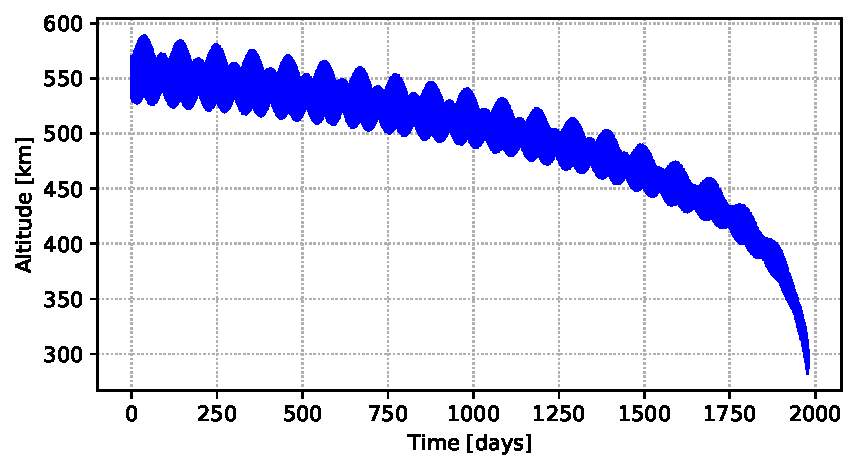
\includegraphics[width=0.8\columnwidth]{figures/lifetime}
        \end{center}
    \end{figure}

\end{frame}

\begin{frame}{Communication Study}

\end{frame}

\begin{frame}{Required Power Budget}

\end{frame}

\begin{frame}{Possible Solutions: Clock Reference}

    \begin{columns}[t]
        \begin{column}[t]{0.65\textwidth}
            \begin{itemize}
                \item Quartz oscillator (XO)
                \vspace{0.1cm}
                \item Temperature Compensated Crystal Oscillators (TCXO)
                \vspace{0.1cm}
                \item Oven Controlled Crystall Oscillators (OCXO)
                \vspace{0.1cm}
                \item Rubidium oscillators (RbXO)
                \vspace{0.1cm}
                \item Cesium oscillators
                \vspace{0.1cm}
                \item GPS disciplined oscillators (GPSDO)
            \end{itemize}
        \end{column}
        \begin{column}[t]{0.4\textwidth}
            \begin{figure}[!ht]
                \begin{center}
                    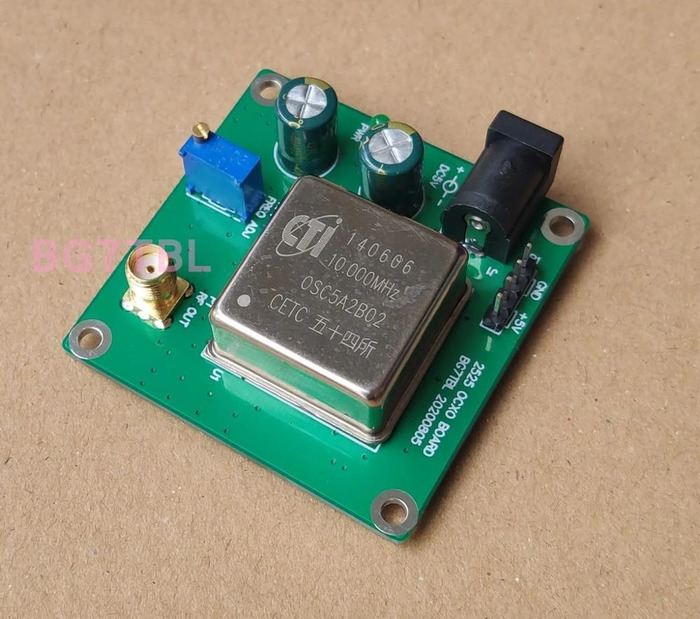
\includegraphics[width=0.8\columnwidth]{figures/ex-ocxo}
                \end{center}
            \end{figure}

            \begin{figure}[!ht]
                \begin{center}
                    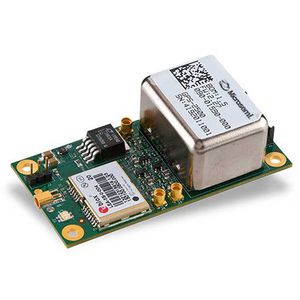
\includegraphics[width=0.8\columnwidth]{figures/gps-2550}
                \end{center}
            \end{figure}
        \end{column}
    \end{columns}

\end{frame}

\begin{frame}{Comparison Between Clock Reference Types}

    \begin{table}[!ht]\tiny
        \centering
        \begin{tabular}{lcccc}
            \toprule[1.5pt]
            \textbf{Oscillator Type} & \textbf{Accuracy} & \textbf{Aging/10 year} & \textbf{Power} & \textbf{Weight} \\
            \midrule
            XO                   & $10^{-5}$ to $10^{-4}$   & 10-20 PPM                                 & 20 $\mu$W  & 20 g \\
            TXCO                 & $10^{-6}$                & 2-5 PPM                                   & 100 $\mu$W & 50 g \\
            MCXO                 & $10^{-8}$ to $10^{-7}$   & 1-3 PPM                                   & 200 $\mu$W & 100 g \\
            OCXO (5 to 10 MHz)   & $10^{-8}$                & $2 \times 10^{-8}$ to $2 \times 10^{-7}$  & \multirow{2}{*}{1-3 W} & \multirow{2}{*}{200-500 g} \\
            OCXO (15 to 100 MHz) & $5 \times 10^{-7}$       & $5 \times 10^{-10}$ to $5 \times 10^{-9}$ &            &  \\
            RbXO                 & $10^{-9}$                & $5 \times 10^{-10}$ to $5 \times 10^{-9}$ & 6-12 W & 1,5-2,5 kg\footnote{There are miniaturized versions.} \\
            Cs                   & $10^{-12}$ to $10^{-11}$ & $10^{-12}$ to $10^{-11}$                  & 25-40 W & 10-20 kg \\
            GPS                  & $4 \times 10^{-8}$ to $10^{-11}$ & $10^{-13}$ & 4 W & 340 g \\
            \bottomrule[1.5pt]
        \end{tabular}
        \label{tab:osc-comp}
    \end{table}

\end{frame}

\begin{frame}{Chip Scale Rubidium Oscillator (RbXO)}

    \begin{columns}[t]
        \begin{column}[t]{0.65\textwidth}
            \begin{itemize}
                \item \textbf{Model}: Microchip CSAC-SA-45S
                \vspace{0.2cm}
                \item \textbf{Power consumption}: 120 mW
                \vspace{0.2cm}
                \item \textbf{Volume}: 17 cm$^{3}$
                \vspace{0.2cm}
                \item \textbf{Weight}: 35 g
                \vspace{0.2cm}
                \item \textbf{Accuracy}: $\pm 5 \times 10^{-11}$
                \vspace{0.2cm}
                \item \textbf{Operating temperature}: -10 to 70$^{\circ}$C
            \end{itemize}
        \end{column}
        \begin{column}[t]{0.5\textwidth}
            \begin{figure}[!ht]
                \begin{center}
                    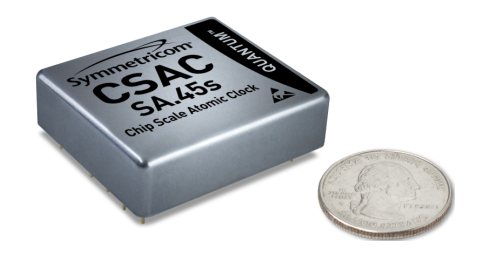
\includegraphics[width=\columnwidth]{figures/microchip-csac}
                \end{center}
            \end{figure}
        \end{column}
    \end{columns}

\end{frame}

\begin{frame}{Possible Solutions: Radio transmitters, Antennas and Attitude and Orbit Control}

\end{frame}

\begin{frame}{Proposed Experiment}

    \begin{itemize}
        \item .
    \end{itemize}

\end{frame}

\begin{frame}{Proposed Experiment}

    \begin{figure}[!ht]
        \begin{center}
            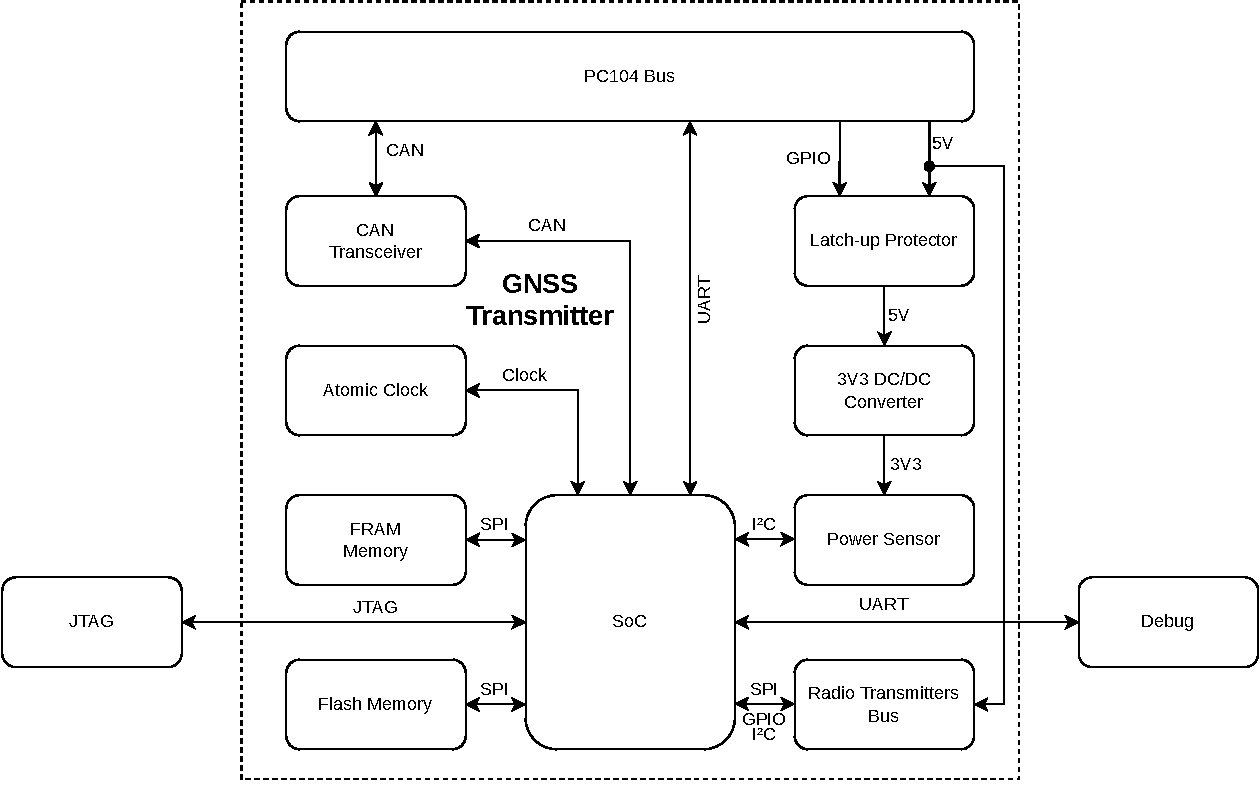
\includegraphics[scale=0.5]{figures/block-diagram}
        \end{center}
    \end{figure}

\end{frame}

\begin{frame}{Proposed Experiment}

    \begin{figure}[!ht]
        \begin{center}
            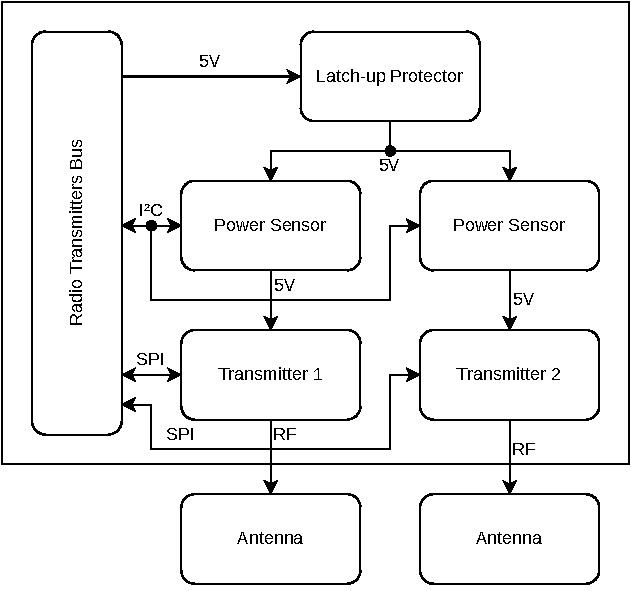
\includegraphics[scale=0.55]{figures/radios-block-diagram}
        \end{center}
    \end{figure}

\end{frame}


    \section{Next Steps}

        %
% future.tex
%
% Copyright (C) 2023 by Gabriel Mariano Marcelino.
%
% Towards the Conception of GNSS Networks Based on Small Satellites
%
% This work is licensed under the Creative Commons Attribution-ShareAlike 4.0
% International License. To view a copy of this license,
% visit http://creativecommons.org/licenses/by-sa/4.0/.
%

%
% \brief Next steps slides.
%
% \author Gabriel Mariano Marcelino <gabriel.mm8@gmail.com>
%
% \version 1.0.0
%
% \date 2023/09/09
%

\begin{frame}{Next Steps}

    \begin{itemize}
        \item An orbit analysis will be performed to determine the minimum number of satellites required for different types of orbits
        \vspace{0.1cm}
        \item A trade-off analysis will be performed to evaluate the complexity of each satellite and the constellation versus the operational orbit of the system
        \vspace{0.1cm}
        \item The proposed payload will also be developed for a possible future implementation and deployment in one of the research group's upcoming missions. A mission composed of multiple satellites will also be presented and proposed
        \vspace{0.1cm}
        \item The publication of at least one paper about this work is also planned
    \end{itemize}

\end{frame}


    \sectionpic{Thanks!}{figures/brazil-south.jpeg}

\end{document}
